\documentclass{article}
\usepackage{graphicx}
\usepackage{float}
\usepackage[margin=.75in]{geometry}

\usepackage{hyperref}
\hypersetup{
    colorlinks=true,
    linkcolor=blue,
    filecolor=magenta,      
    urlcolor=cyan,
}
 
\urlstyle{same}
\begin{document}

Code used in production of plots for this section can be found at https://github.com/cfmcginn/SystBio/tree/master/HW10.

\section{2.a-c}

In Fig.~\ref{fig:fig1} left hand side is plotted the popuation of winning genes where fixation requires acheiving a size ten, while the right hand side shows the winning genes when the population size is 500. Since in size ten case we are at such a small population, none of the mutation rates make a sizable impact. Survival is purely stochastic, an effective 50-50 coin flip for all introduced mutants relative each other. Hence all distributions track the underlying distribution more or less exactly

In the right-hand side of Fig.~\ref{fig:fig1} we see that at large population sizes, the different gene success probabilities can assert themselves, and the mutation rate of 0 and 0.00002 peaks at s0 of 0.02, the characteristic value of the exponential distirbution we draw values from. This matches expectations, as if we integrate the exponential distribution over the win probability in this regime (simply the s0), we get the mean of the exponential which is its characteristic parameter. Note that the mutation rates of 0 and 0.00002 perfectly overlap, as expected. Clonal interference should only shift the distribution upward in the limit that mutation rate times population size is greater than 1. This is true for the 0.01 case, and we see the appropriate shift. 

\begin{figure}[H]
    \centering
    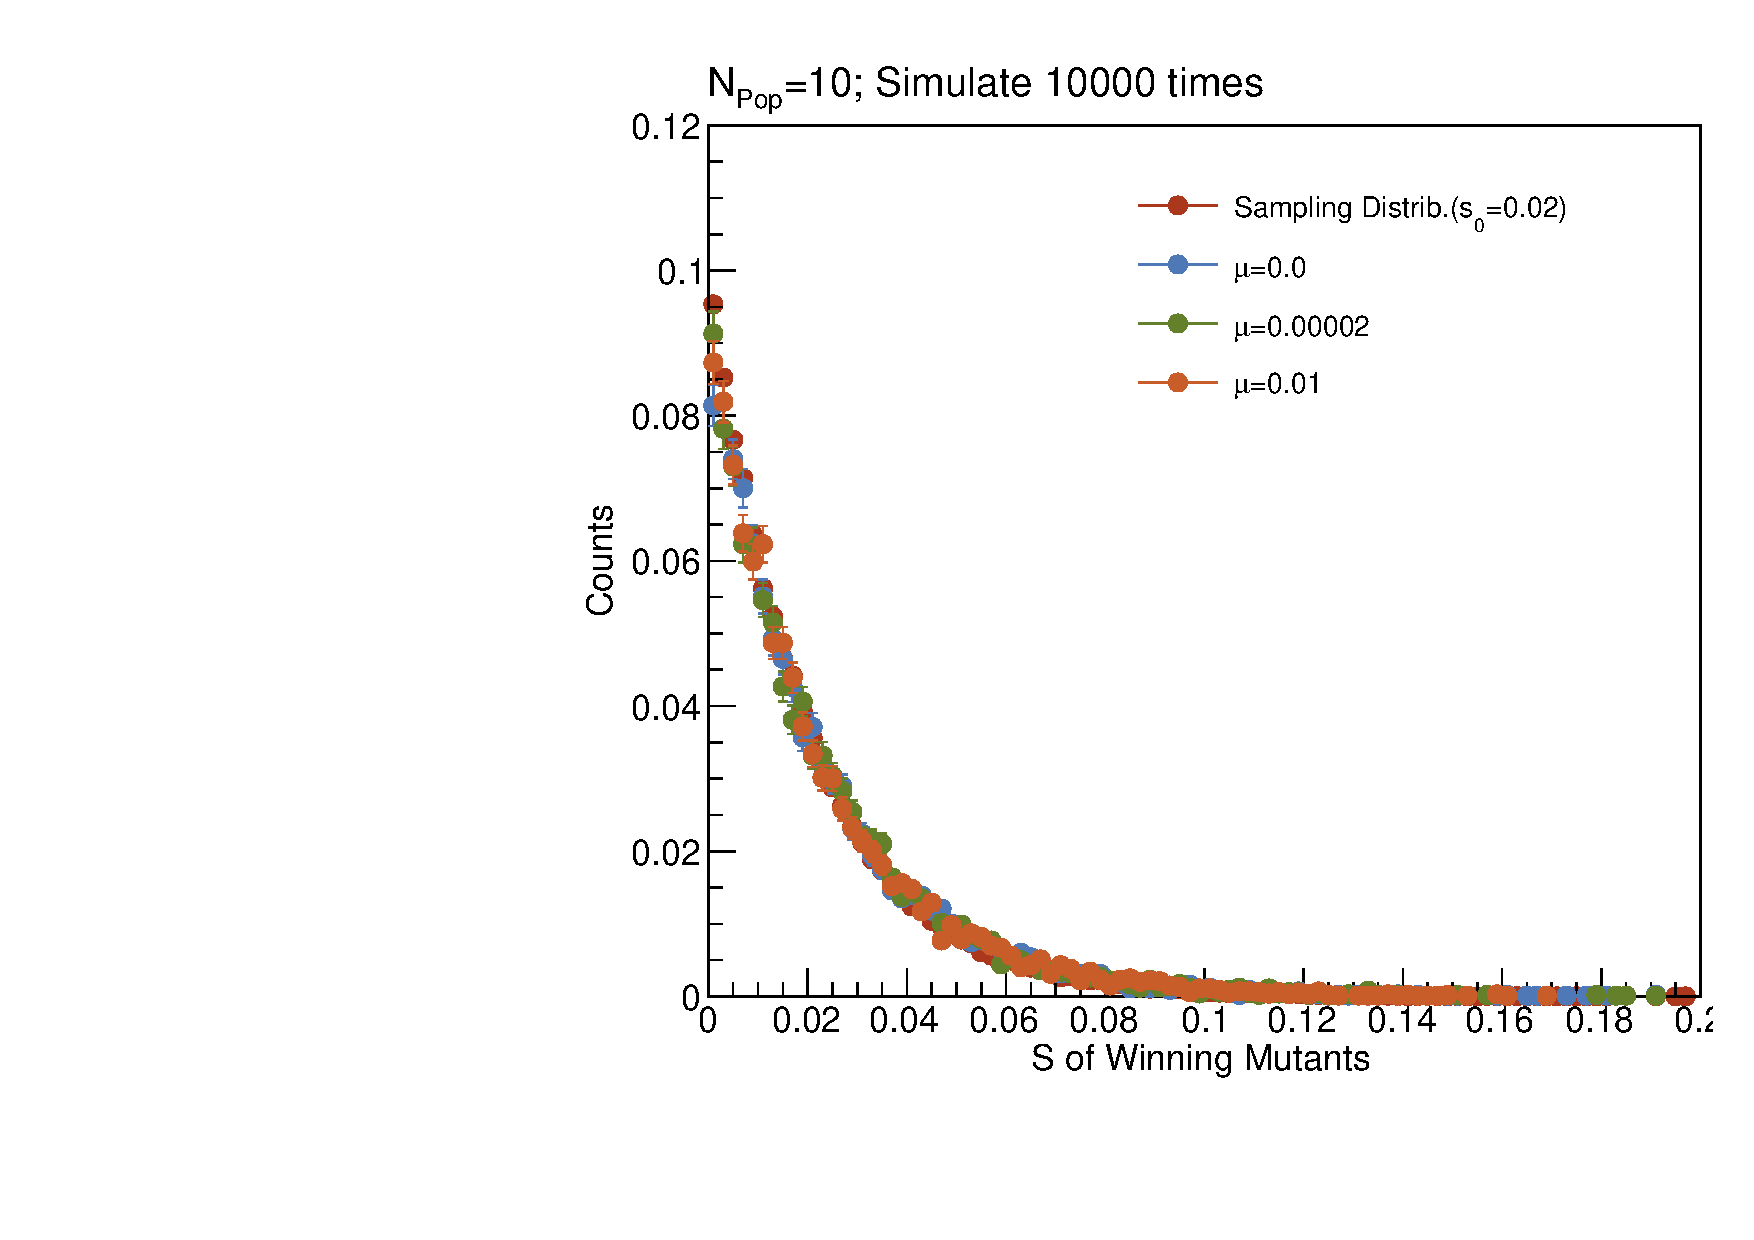
\includegraphics[width=.45\textwidth]{plotMoran_NPop10.pdf}
    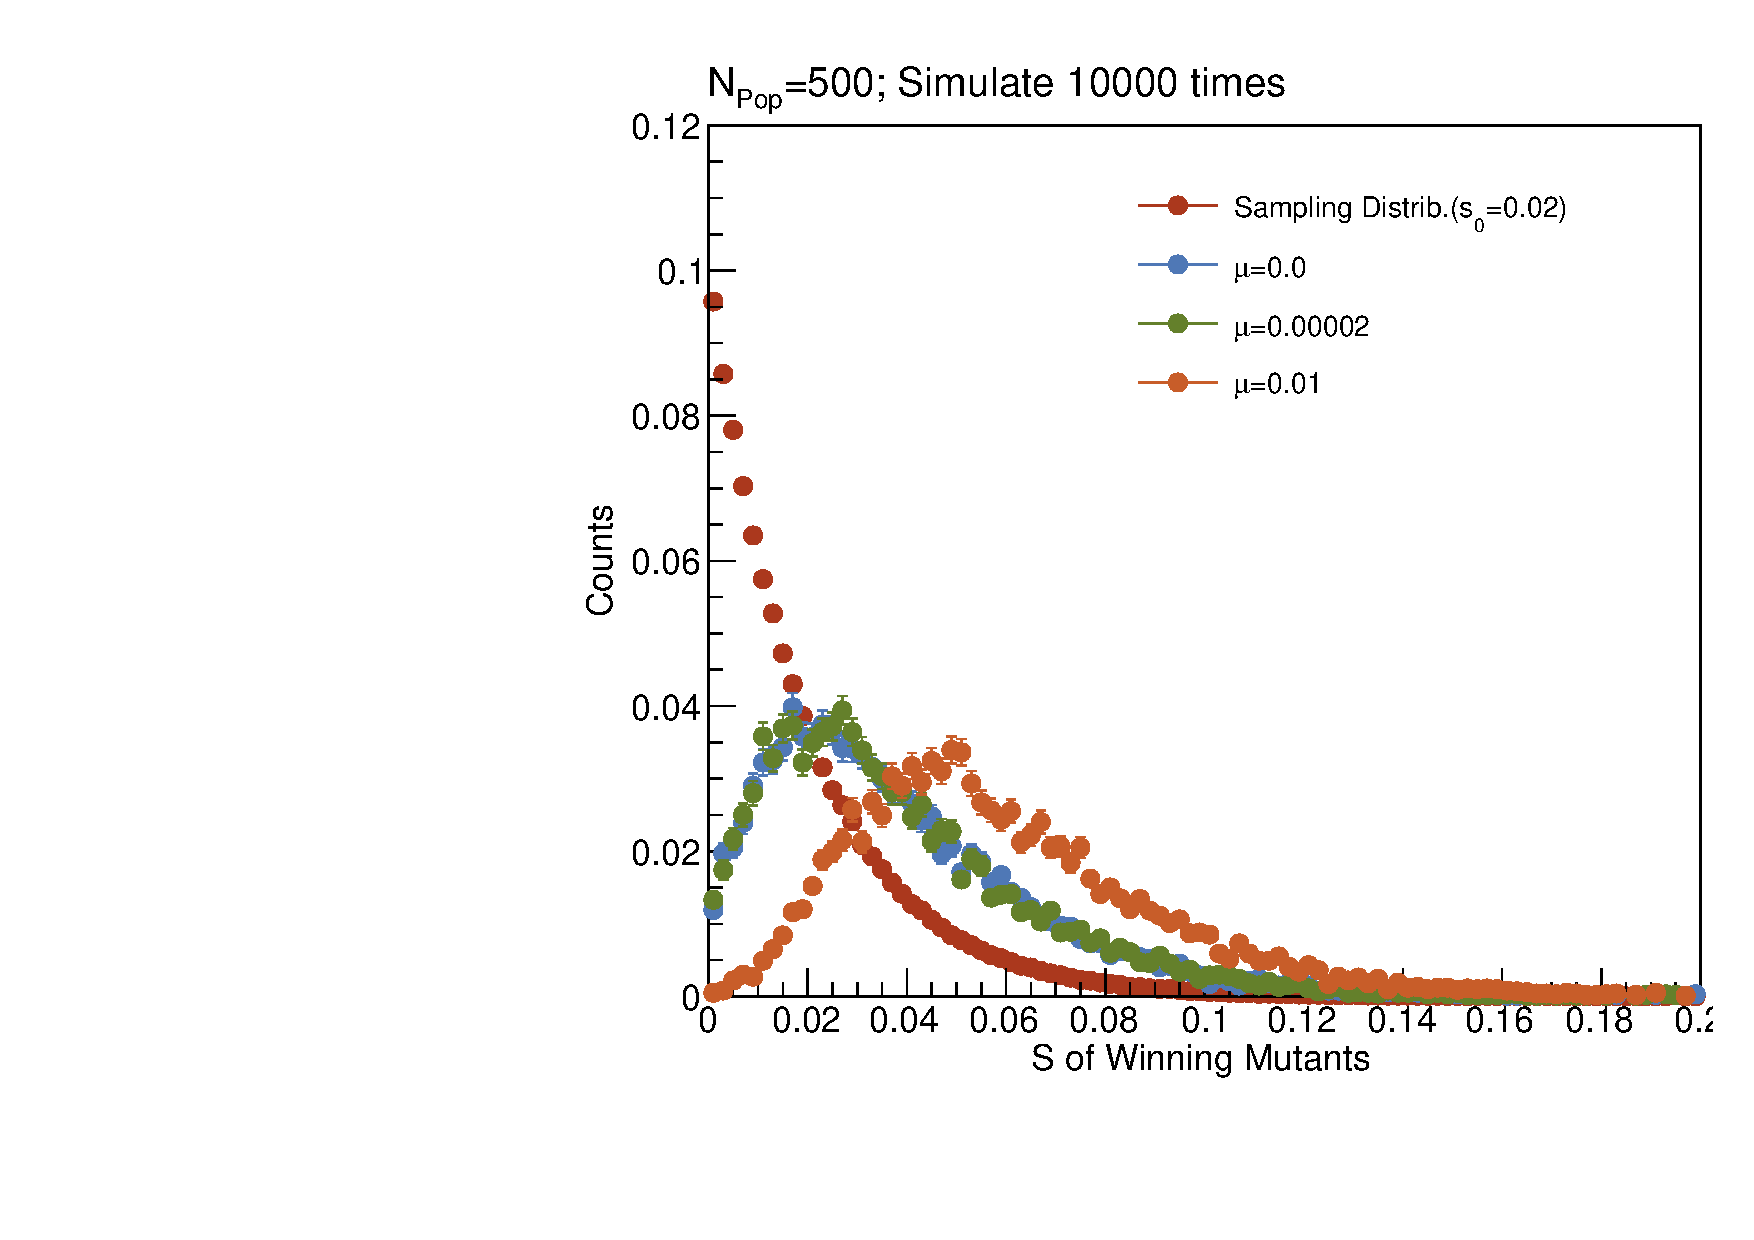
\includegraphics[width=.45\textwidth]{plotMoran_NPop500.pdf}
    \caption{Left: Plot of underlying fitness distribution (exponential w/ characteristic value s0=0.02) along with distribution of winning fitnesses with various mutation rates for N = 10. Right: The same is plotted as the left-hand side but with N = 500.}
    \label{fig:fig1}
\end{figure}

\section{3.c}

The expectation for l(k) is 1.025, but the expectation for log(l(k)) is -.1023. Since this model is the multiplication of many factors with some mean expectation sub 1 in multiplication, we see that the mean and median diverge. This is because while the overwhelming majority of cases tend towards zero, we develop some long tail of very high values that bias the mean upwards. In this context the mean is not a reasonable characterization of the distribution. See Fig.~\ref{fig:fig2} left hand side for these pockets of higher values at t of 300 seconds and Fig.~\ref{fig:fig3} for the evolution of the mean and median with time.

\begin{figure}[H]
    \centering
    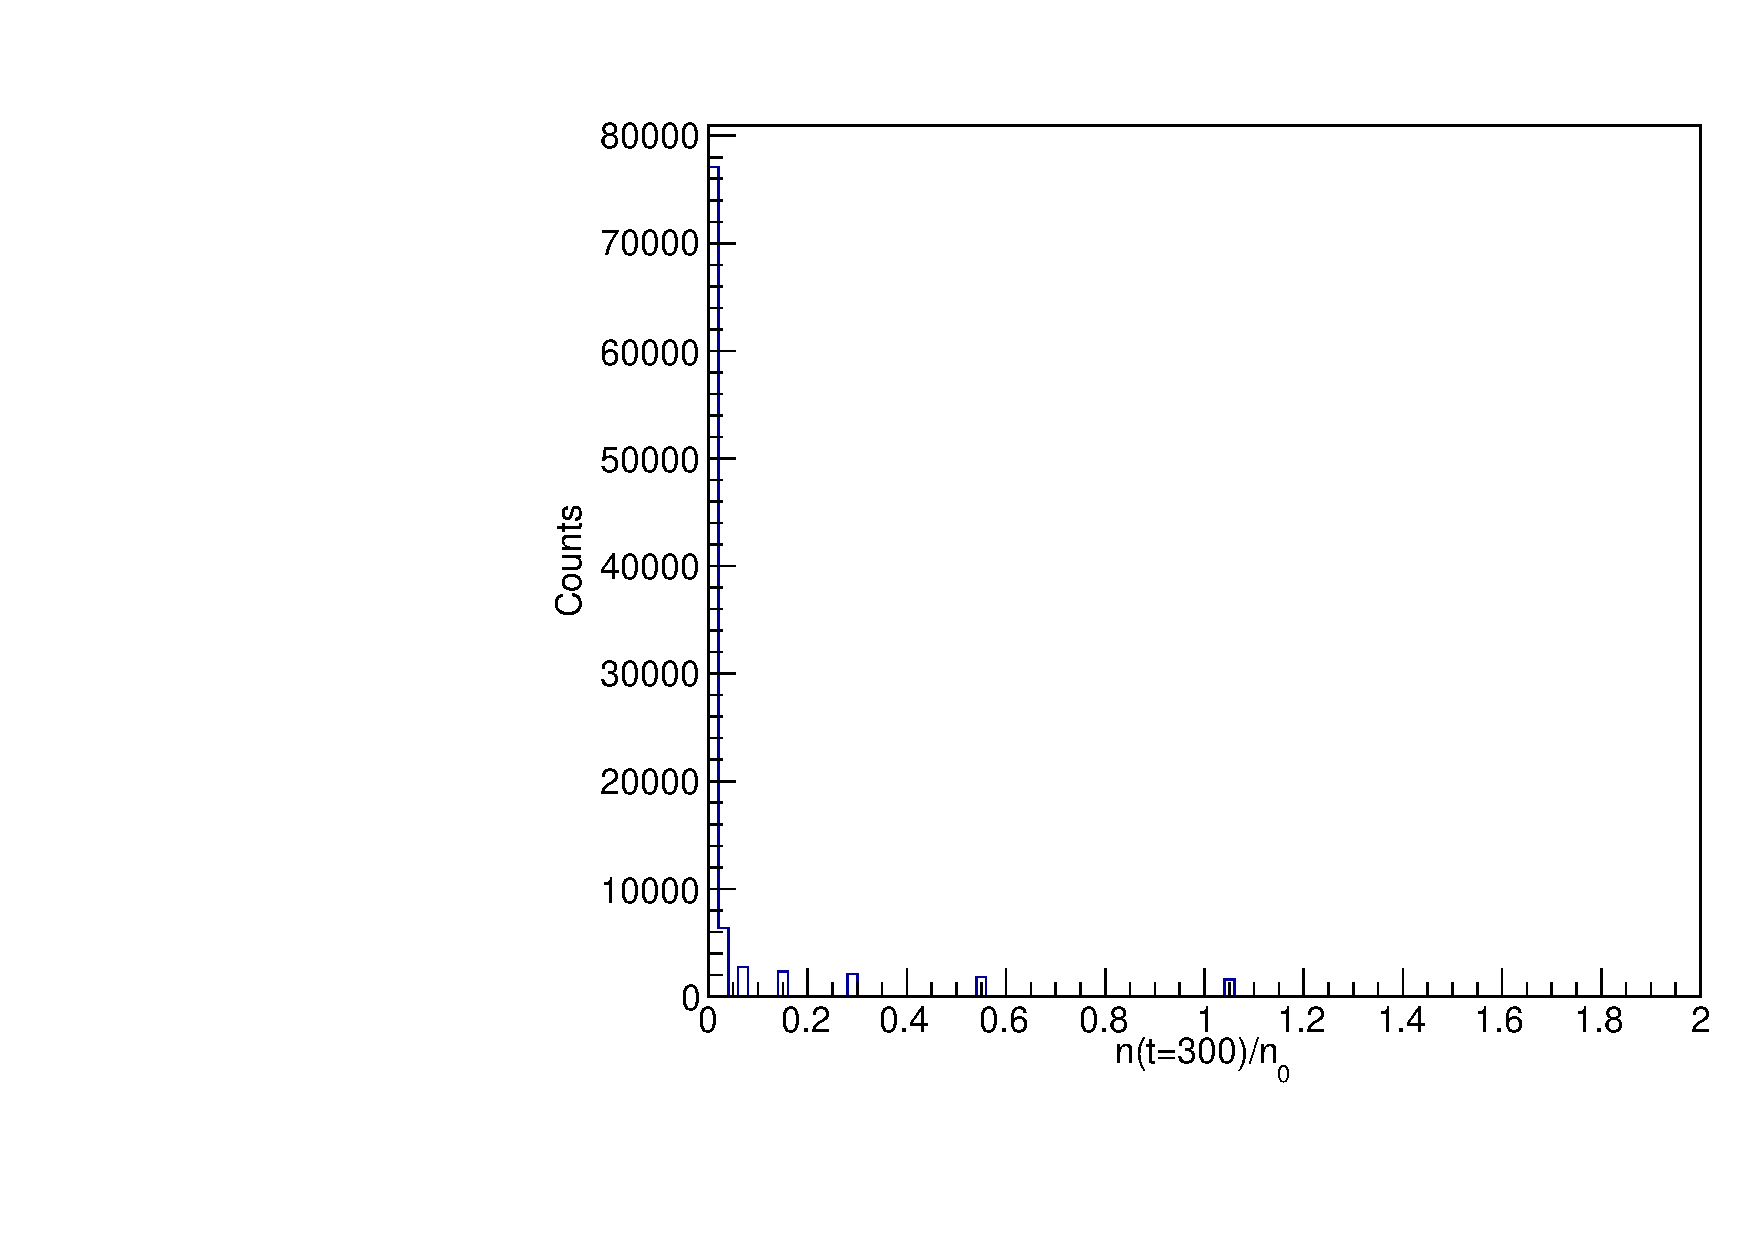
\includegraphics[width=.45\textwidth]{betHedge300Hist.pdf} 
    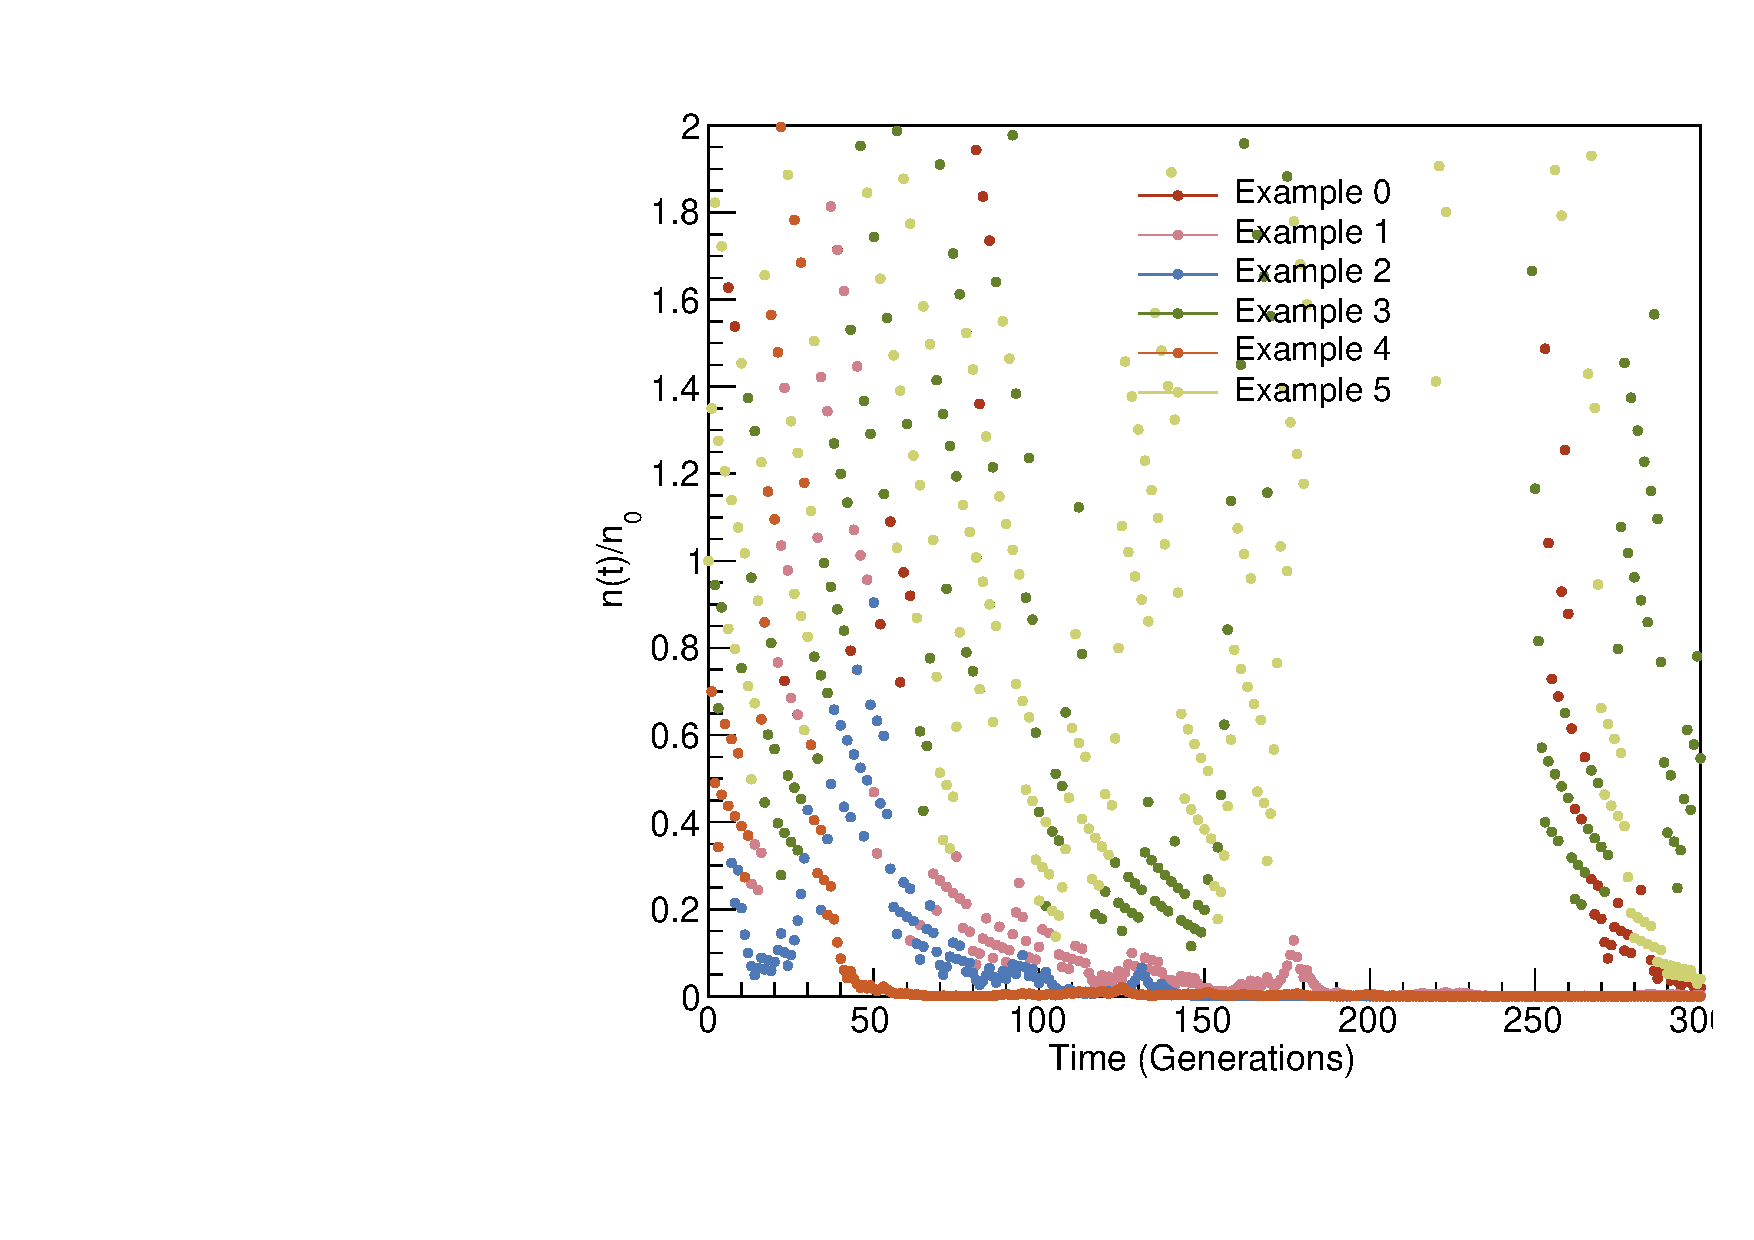
\includegraphics[width=.45\textwidth]{timeSeriesBetHedge.pdf} 
    \caption{Left: The distribution of number of seeds after 300 iterations for 100000 simulations. Note it is strongly peaked at 0 but has pockets of larger numbers. Right: A few examples of individual time series and their evolution.}
    \label{fig:fig2}
\end{figure}

\begin{figure}[H]
    \centering
    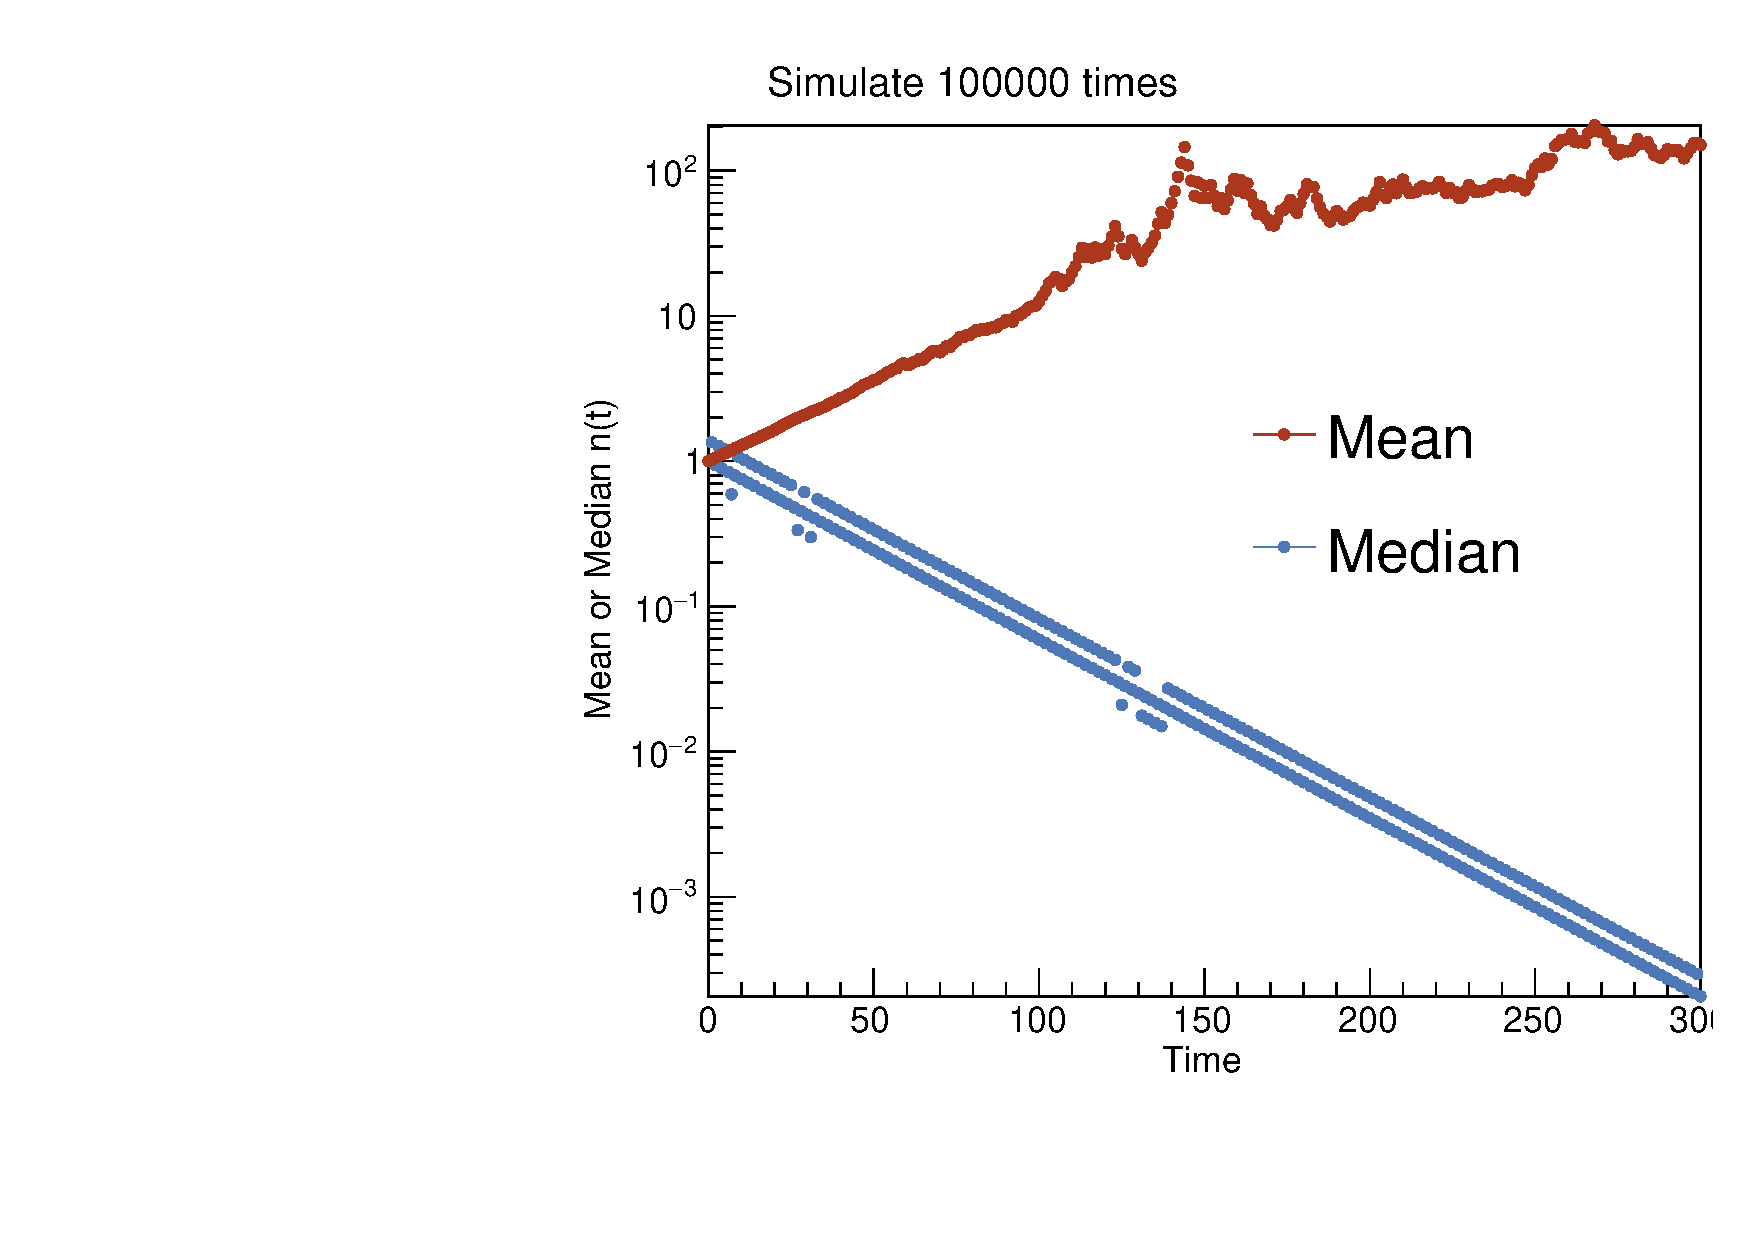
\includegraphics[width=.7\textwidth]{betHedgeMeanMedian.pdf} 
    \caption{Plot of mean and median number of seeds of 100000 simulations per time step for 300 time steps. The divergence of mean and median is due to small numbers of very large numbers of seeds, the overwhelming majority of simulations tend towards zero, as showin in Fig.~\ref{fig:fig2}, left.}
    \label{fig:fig3}
\end{figure}

\end{document}

